\documentclass{article}
\usepackage[utf8]{inputenc}
\usepackage{graphicx} 
\title{Introduction to Philosophy: God, Knowledge and Consciousness}
\author{Huynh Xuan Phung - edX}
\date{ }
\usepackage{color}   %May be necessary if you want to color links
\usepackage{hyperref}
\hypersetup{
    colorlinks=true, %set true if you want colored links
    linktoc=all,     %set to all if you want both sections and subsections linked
    linkcolor=blue,  %choose some color if you want links to stand out
} 
\begin{document}
 
\maketitle
 
\tableofcontents
\section{God}


\subsection{What is Philosophy?}
Philosophical questions are (i) general, (ii) important to all people (iii) such that there are no agree upon methods of answering them.

When looking to prove the existence (or non-existence) of God, people would persuade any reasonable person that God does (or does not) exist just by appealing to what we all already know.

According to Anselm: God, by definition, is so great that it not possible to think of anything greater.

Anselm classifies everything into two domains: Thing that Exist in the Understanding and Thing that Exist in Reality

\begin{figure}
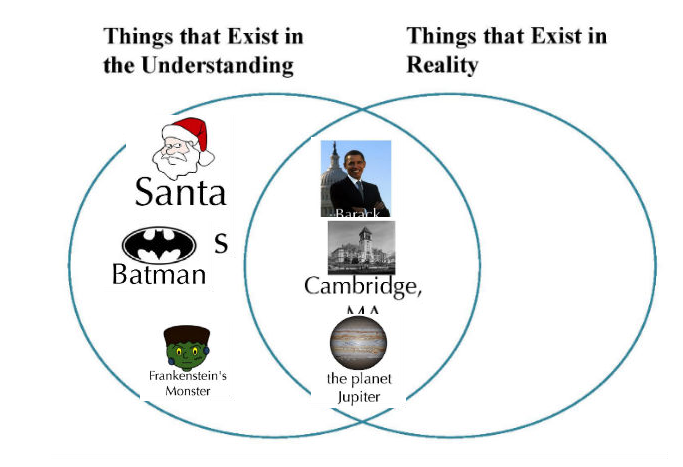
\includegraphics[scale=0.6]{figures/Understanding_Reality.png}
\caption{Examples of Anselm's way of classifying different ways for things to exist.}
\end{figure}


\subsection{Does God exist?}

if God existed only in the Understanding, then we could think of something greater than him: something just like him, but existing in both the Understanding and Reality. But we can't think of something greater than God, so God must not exist only in the Understanding.

\pagebreak


\section{Assessing Arguments}

\subsection{What is an Argument?}
An argument is a list of claims, all but the last of which are labeled "premises", the las of which is tagged a "conclusion".

\subsection{Validity Argument}
An argument is valid if and only if it is impossible for all its premises to be true and its conclusion false.


\subsection{Soundness Argument}
An argument is sound if only if it is valid and al its premises are true

\subsection{Potential Convincingness}
An argument is potential convincing for a person if only if she or he is in a position to see that the argument is valid, and prior to being confronted with the argument, believes the premises but not the conclusion.

\subsection{Applying for persuade that God exists}
\begin{itemize}
\item{P1: Either God exists in the understanding but not in reality or God exists in the understanding and reality}
\item{P2: If God exists in the understanding but not in reality, then we can conceive of thing greater than God(a thong different in virtue of existing in the understanding and reality, but otherwise like God)}
\item{P3: It is not the case that we can conceive of a thing greater than God}

\item{C: God exists in the understanding and in reality}
\end{itemize}

\pagebreak

\section{Argument from the Design}

You find a watch. You might have for thinking that it was designed by somebody because its parts are almost perfectly suited to support the function of the whole.

\subsection{Inference to the best explanation}

If you have some evidence. There are different explanations of how the evidence came to be. You see that one explanation is better than the others. Then you should believe that explanation is likely correct.
\subsection{White's Analogy}

Our existence was dependent on cosmological constants having just the right values and we observe that we exist. I should think somebody who wanted creates like us to be alive.

\subsection{The Fine-Tuning Argument}
Roger White's Fine-Tuning Argument for the existence of God

P1: Inference to the Best Explanation: If a face E that we observe stands in need of explanation, and hypothesis H provides a satisfactory explanation of E and one that is the better than any alternative explanation available, then E provides significant evidential support for H.

P2: That our universe is hospitable to life stands in need of explanation

P3: That God adjusted the constants in order to allow for life to develop provides a satisfactory explanation for why our universe is hospitable to life

P4: There is no comparably satisfying explanation of this fact available

--------------------------------

C: That our universe is hospitable to life provides significant evidential support for the hypothesis that God adjusted the constants

IF there is a universe in which the physical constants are different, then the fact that our universe is hospitable to life does not call out for an explanation

Everything is antecedently even though it is not valuable for you (need an explanation) but for someone, it is enough valuable to need an explanation.

\section{Against God: the Problem of Evil}

\subsection{Omniscient, Omni-benevolent, Omnipotent God}

Omniscience: Everything you believe to be tree is true. Everything that is true you believe to be true.

Omni-benevolence, when:
--- 1. For each of us, it wants as to be better off rather than worse off
--- 2. Given a choice between the world being better and worse, it always wants the world to be better.

Omnipotence, when:
--- 1. Everything that it wants to be the case is the case
--- 2. If it were to want anything to be the case then it would be the case

The conclusion of the Problem of Evil Argument is that a very particular kind of God doesn't exist. It aims to show that there is no omniscient, omni-benevolent, and omnipotent God


\subsection{The Problem of Evil}
 
The reconstruction of the Problem of Evil Argument

---P1. Some terrible things happen

---P2. If there were and omniscient, omnibenevolent, omnipotent God, then no terrible things would happen

-----------------------------------------------

---C. There is no omniscient, omnibenevolent, omnipotent God.



\subsection{This is the Best of All Possible Worlds}

Why might an omnibenevolent God have wanted terrible things to happen?

The Causal Ideal: God wanted the terrible things to happen because the terrible things caused the many good things to happen.

The Constitutive idea: God wanted the terrible things to happen because part of what makes good things good is the existence of terrible things

\subsection{Terror is the Price of Freedom}

\subsection{There is no Best Possible World}

There is no best possible world. For any possible world there is a better one.

\section{Pascal's Wager}
\subsection{Epistemic and Practical Reasons for Belief}

A practical reason for you to believe that Q is a consideration that gives you evidence that it is in your interests to believe that Q.

--- Example of consideration that gives you evidence that you will be happy if you believe that your flavored politician will win. And it is of course in your interests to be happy

A Epistemic Reason for you to believe that Q is a consideration that give you evidence that it is the case that Q.

--- The face that your flavored politician is ahead in all the polls gives you evidence that your flavored politician will win.

\subsection{Pascal's Wager}

As follow

P1: It is always rational for you to take the option open to you with highest expected value

P2: For you, believing in God has higher expected value than not believing in God

-------------------------------------------------------

C It is rational for you to believe in God


A Finite Rewards: You have a better, irreligious life here on earth, not worrying about prayer, church tithes, ...

An Infinite Rewards: You spend eternity in Heaven


Expected value: $E(option_a) = \sum_{Outcome_1}^{Outcome_n} P (Outcome_i/ option_a)* Value(Outcome_i)$


\end{document}